\chapter{Desenvolvimento}
Neste capítulo são apresentados a metodologia e detalhes sobre o desenvolvimento do trabalho.
Nos itens deste capítulo será apresentada a metodologia e detalhado o desenvolvimento do software da biblioteca,
demonstrando requisitos, arquitetura, ambiente de implementação, documentação e implementação.


\section{Metodologia}
topico pequeno enchendo linguiça


\section{Requisitos da Biblioteca}

O levantamento de requisitos e concepção inicial da dinâmica e uso da biblioteca, foi realizado com base no caminho de
acesso as funcionalidades que um usuário da biblioteca faria, de forma a levar em conta os objetivos específicos
propostos na introdução do trabalho.

O resultado da análise foi o seguinte diagrama de casos de uso, que denota um caminho provável de ações do usuário:

\begin{figure}[H]
    \centering
    \caption{Casos de uso}
    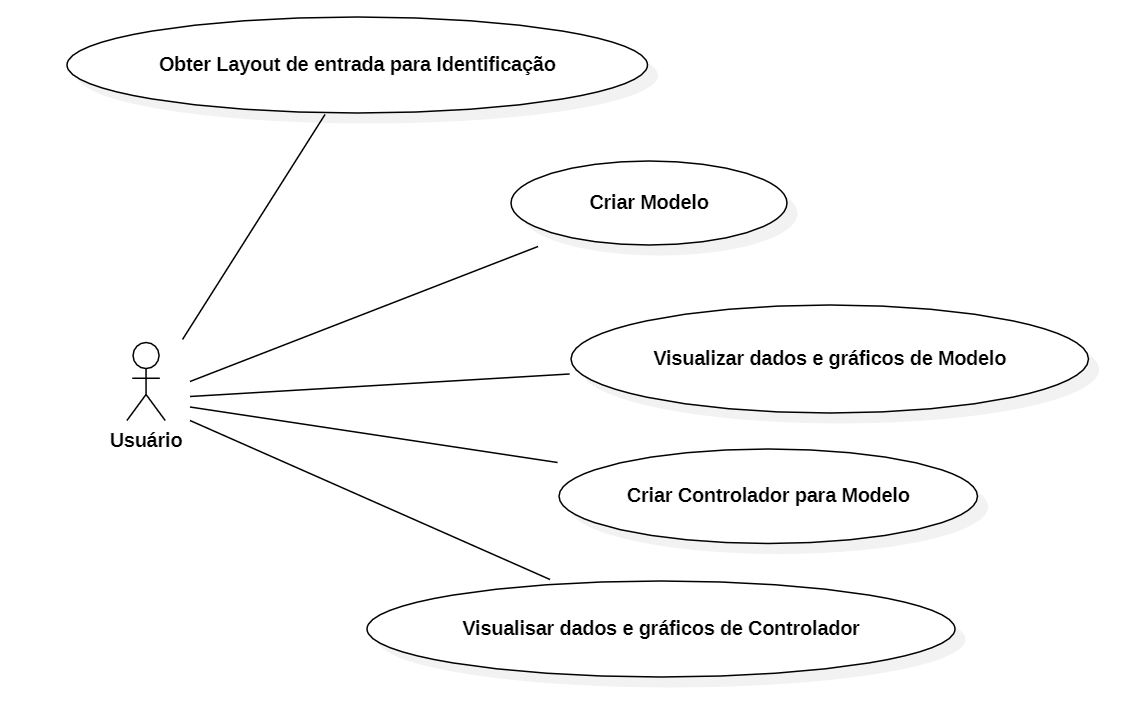
\includegraphics[scale=0.5]{figuras/use_cases}
    \label{fig:use_cases}
    \\
    \vspace{0cm}\hspace{0cm}\small{Fonte: Do autor}
\end{figure}

As tabelas \ref{tab:uc1}, \ref{tab:uc2}, \ref{tab:uc3}, \ref{tab:uc4}, \ref{tab:uc5} detalham os casos de uso ilustrado
na figura \ref{fig:use_cases}, especificando o objetivo, os pré requisitos e o cenário de cada caso de uso.


\begin{table}[!htbp]
    \begin{center}
        \begin{tabularx}{\textwidth}{|>{\bfseries\raggedright\arraybackslash\center}m{5cm}|X|}
            \hline
            Identificador UC: UC-1\newline Diagrama ID: D-1 & Nome: Obtenção de layout de input de dados para identificação\newline Prioridade: Alta                                                                                                                                                                                                   \\ \hline
            Objetivo                                        & Fornecer planilha de layout para que sejam inseridos os dados necessários para um determinado processo de identificação.                                                                                                                                                                 \\ \hline
            Atores                                          & Usuário                                                                                                                                                                                                                                                                                  \\ \hline
            Restrições                                      & Deve-se salvar a planilha referente ao layout necessário.                                                                                                                                                                                                                                \\ \hline
            Pré-condições                                   & -                                                                                                                                                                                                                                                                                        \\ \hline
            Cenário principal                               & 1. O método é chamado, recebendo o caminho onde deve salvar o arquivo e possívelmente os parâmetros referentes ao layout em espessífico, como tipo de arquivo, por exemplo.\newline 2. É construido em memória o layout desejado.\newline 3. É salvo o arquivo no caminho espessificado. \\ \hline
            Pós condições                                   & O Usuário possui o layout e pode inserir os dados.                                                                                                                                                                                                                                       \\ \hline
        \end{tabularx}
        \caption{Obtenção de layout de input de dados para identificação}
        \label{tab:uc1}
    \end{center}
\end{table}

\begin{table}[!htbp]
    \begin{center}
        \begin{tabularx}{\textwidth}{|>{\bfseries\raggedright\arraybackslash\center}m{5cm}|X|}
            \hline
            Identificador UC: UC-2\newline Diagrama ID: D-2 & Nome: Indentificação de sistema\newline Prioridade: Alta                                                                                                                                                                                                                                             \\ \hline
            Objetivo                                        & Realizar processo de identificação do sistema baseado nos dados e obter modelo.                                                                                                                                                                                                                      \\ \hline
            Atores                                          & Usuário                                                                                                                                                                                                                                                                                              \\ \hline
            Restrições                                      & Deve-se obter o modelo do sistema.                                                                                                                                                                                                                                                                   \\ \hline
            Pré-condições                                   & layout de dados preenchido.                                                                                                                                                                                                                                                                          \\ \hline
            Cenário principal                               & 1. O método de identificação é chamado, recebendo o caminho do arquivo de layout e possívelmente os parâmetros referentes ao método em espessífico.\newline 2. São realizados os cálculos e é obtido o objeto de modelo do sistema.\newline 3. O objeto de modelo do sistema é retornado ao usuário. \\ \hline
            Pós condições                                   & O Usuário possui um objeto de modelo do sistema.                                                                                                                                                                                                                                                     \\ \hline
        \end{tabularx}
        \caption{Indentificação de sistema}
        \label{tab:uc2}
    \end{center}
\end{table}

\begin{table}[!htbp]
    \begin{center}
        \begin{tabularx}{\textwidth}{|>{\bfseries\raggedright\arraybackslash\center}m{5cm}|X|}
            \hline
            Identificador UC: UC-3\newline Diagrama ID: D-3 & Nome: Visualização de modelo de sistema\newline Prioridade: Alta                                                                                                                                                                                                                         \\ \hline
            Objetivo                                        & Visualizar gráfico e dados indicadores importantes de um modelo.                                                                                                                                                                                                                         \\ \hline
            Atores                                          & Usuário                                                                                                                                                                                                                                                                                  \\ \hline
            Restrições                                      & Deve ser possível visualisar gráfico e dados indicadores importantes do modelo.                                                                                                                                                                                                          \\ \hline
            Pré-condições                                   & O Usuário possui um objeto de modelo do sistema.                                                                                                                                                                                                                                         \\ \hline
            Cenário principal                               & 1. Um método de visualisação de dados ou gráfico é chamado, passando possíveis parâmetros necessários ou que irão mudar a forma como os dados serão exibidos.\newline 2. São preparados os objetos a serem exibidos ao usuário.\newline 3. São exibidos os dados ou gráficos ao usuário. \\ \hline
            Pós condições                                   & O Usuário pode visualisar os dados do modelo.                                                                                                                                                                                                                                            \\ \hline
        \end{tabularx}
        \caption{Visualização de modelo de sistema}
        \label{tab:uc3}
    \end{center}
\end{table}

\begin{table}[!htbp]
    \begin{center}
        \begin{tabularx}{\textwidth}{|>{\bfseries\raggedright\arraybackslash\center}m{5cm}|X|}
            \hline
            Identificador UC: UC-4\newline Diagrama ID: D-4 & Nome: Aproximação de Controlador baseado em modelo de sistema\newline Prioridade: Alta                                                                                                                                                                                                     \\ \hline
            Objetivo                                        & Obter aproximação de parâmetros de controle baseados no modelo obtido.                                                                                                                                                                                                                     \\ \hline
            Atores                                          & Usuário                                                                                                                                                                                                                                                                                    \\ \hline
            Restrições                                      & Deve-se obter uma aproximação dos parâmetros do controlador.                                                                                                                                                                                                                               \\ \hline
            Pré-condições                                   & O Usuário possui um objeto de modelo do sistema.                                                                                                                                                                                                                                           \\ \hline
            Cenário principal                               & 1. O método de aproximação é chamado, recebendo o modelo do sistema e possívelmente os parâmetros referentes ao método de aproximação em espessífico.\newline 2. São realizados os cálculos e é obtido o objeto de controlador.\newline 3. O objeto de controlador é retornado ao usuário. \\ \hline
            Pós condições                                   & O Usuário possui um objeto de controlador.                                                                                                                                                                                                                                                 \\ \hline
        \end{tabularx}
        \caption{Aproximação de Controlador baseado em modelo de sistema}
        \label{tab:uc4}
    \end{center}
\end{table}

\begin{table}[!htbp]
    \begin{center}
        \begin{tabularx}{\textwidth}{|>{\bfseries\raggedright\arraybackslash\center}m{5cm}|X|}
            \hline
            Identificador UC: UC-5\newline Diagrama ID: D-5 & Nome: Visualização de controlador\newline Prioridade: Alta                                                                                                                                                                                                                               \\ \hline
            Objetivo                                        & Visualizar gráfico e dados indicadores importantes de um controlador.                                                                                                                                                                                                                    \\ \hline
            Atores                                          & Usuário                                                                                                                                                                                                                                                                                  \\ \hline
            Restrições                                      & Deve ser possível visualisar gráfico e dados indicadores importantes do controlador gerado.                                                                                                                                                                                              \\ \hline
            Pré-condições                                   & O Usuário possui um objeto de controlador.                                                                                                                                                                                                                                               \\ \hline
            Cenário principal                               & 1. Um método de visualisação de dados ou gráfico é chamado, passando possíveis parâmetros necessários ou que irão mudar a forma como os dados serão exibidos.\newline 2. São preparados os objetos a serem exibidos ao usuário.\newline 3. São exibidos os dados ou gráficos ao usuário. \\ \hline
            Pós condições                                   & O Usuário pode visualisar os dados do controlador.                                                                                                                                                                                                                                       \\ \hline
        \end{tabularx}
        \caption{Visualização de controlador}
        \label{tab:uc5}
    \end{center}
\end{table}




\section{Descrição da arquitetura}\label{sec:descarc}

A fim de construir uma biblioteca com arquitetura de código compreensível e escalável, optou-se pela orientação
da mesma a classes e objetos.
Baseado nisso e nos casos de uso, foi desenvolvido o diagrama de classes da figura \ref{fig:class_diag}.
Onde foram definidas as seguintes classes:
\begin{alineas}
    \item \textbf{DataInputUtils}: Classe utilitária para a entrada de dados externos - pode ser melhor visualizada na figura \ref{fig:class_diag_diubmi};
    \item \textbf{DataUtils}: Classe utilitária para manipulação de dados em memória - pode ser melhor visualizada na figura \ref{fig:class_diag_dupu};
    \item \textbf{PlotUtils}: Classe utilitária para plot de funções de transferência e outras informações relacionadas - pode ser melhor visualizada na figura \ref{fig:class_diag_dupu};
    \item \textbf{Model}: Classe representativa do Modelo matemático de uma planta de sistemas de controle - pode ser melhor visualizada na figura \ref{fig:class_diag_model};
    \item \textbf{ModelView}: Classe utilizada pra visualização de dados de um objeto da classe Model - pode ser melhor visualizada na figura \ref{fig:class_diag_model};
    \item \textbf{BaseModelIdentification}: Classe utilitária base para Identificação de modelos (Model), herdada por classes que implementam métodos de identificação - pode ser melhor visualizada na figura \ref{fig:class_diag_diubmi};
    \item \textbf{Controller}: Classe representativa do Modelo matemático de uma planta de sistemas de controle em Malha Fechada com Controlador PID - pode ser melhor visualizada na figura \ref{fig:class_diag_controller};
    \item \textbf{ControllerView}: Classe utilizada pra visualização de dados de um objeto da classe Controller - pode ser melhor visualizada na figura \ref{fig:class_diag_controller};
    \item \textbf{BaseControllerAproximation}: Classe utilitária base para aproximação de controladores (Controller), herdada por classes que implementam métodos de aproximação de parâmetros de controlador PID - pode ser melhor visualizada na figura \ref{fig:class_diag_bcacontroller}.
\end{alineas}

\begin{figure}[H]
    \centering
    \caption{Diagrama de classes}
    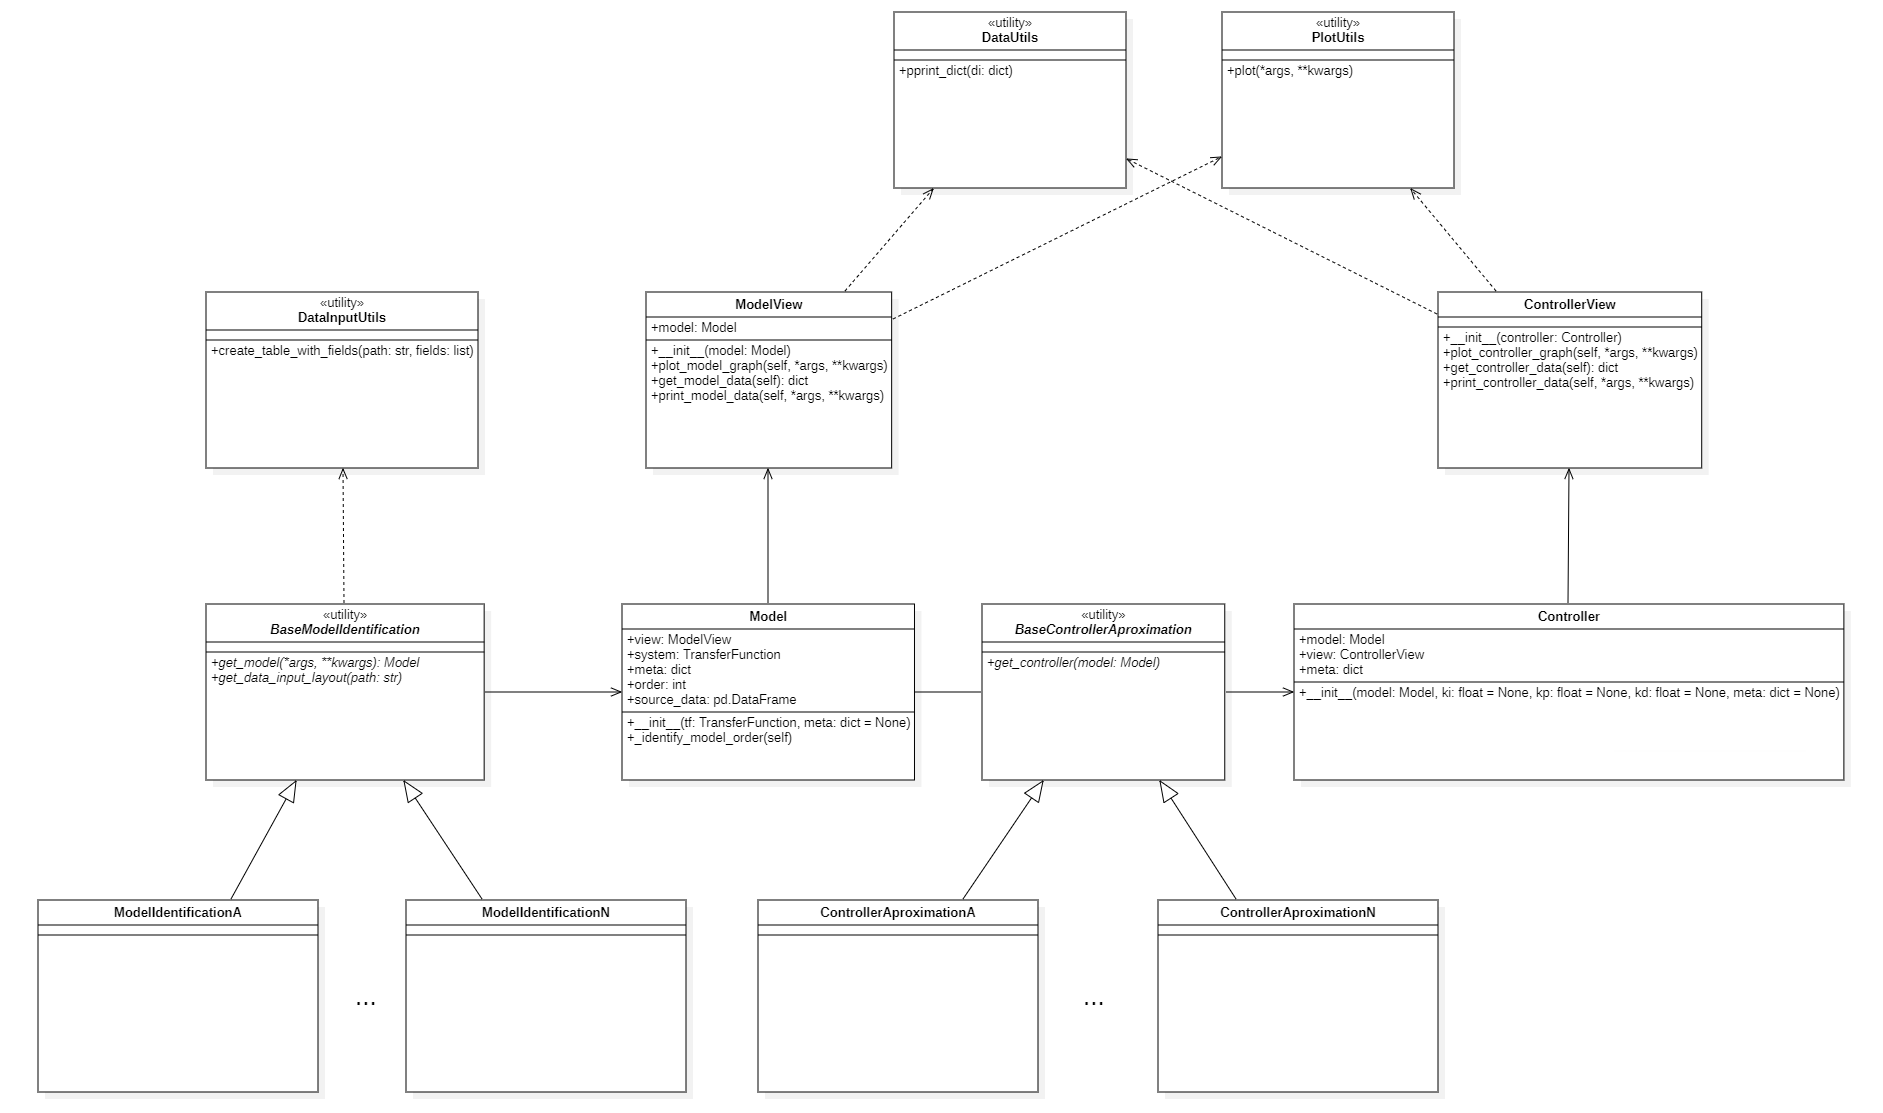
\includegraphics[scale=0.32]{figuras/class_diag}
    \label{fig:class_diag}
    \\
    \vspace{0cm}\hspace{0cm}\small{Fonte: Do autor}
\end{figure}

\begin{figure}[H]
    \centering
    \caption{Diagrama de classes ampliado - DataInputUtils e BaseModelIdentification}
    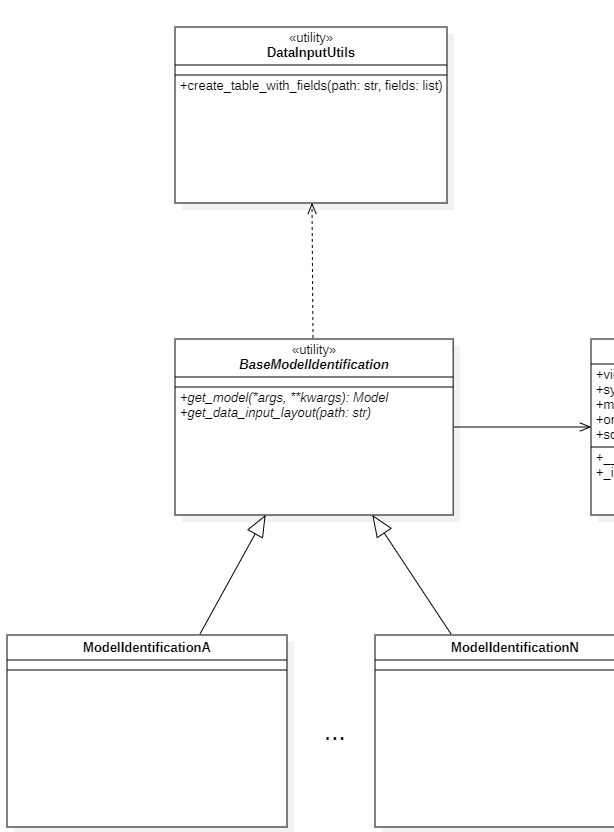
\includegraphics[scale=0.6]{figuras/class_diag_diubmi}
    \label{fig:class_diag_diubmi}
    \\
    \vspace{0cm}\hspace{0cm}\small{Fonte: Do autor}
\end{figure}

\begin{figure}[H]
    \centering
    \caption{Diagrama de classes ampliado - DataUtils e PlotUtils}
    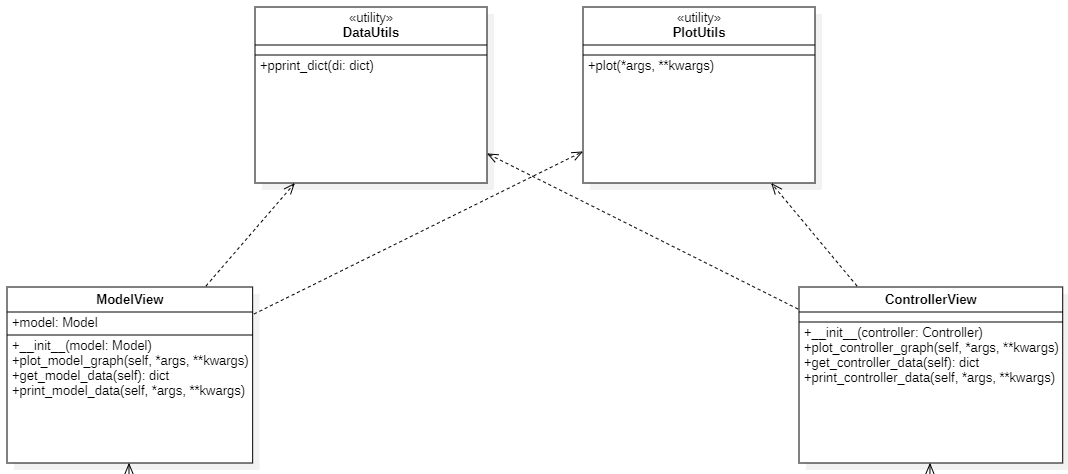
\includegraphics[scale=0.6]{figuras/class_diag_dupu}
    \label{fig:class_diag_dupu}
    \\
    \vspace{0cm}\hspace{0cm}\small{Fonte: Do autor}
\end{figure}

\begin{figure}[H]
    \centering
    \caption{Diagrama de classes ampliado - Model e ModelView}
    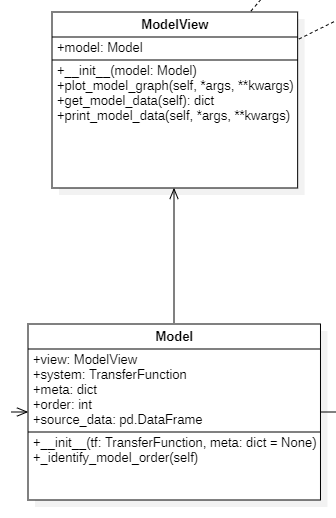
\includegraphics[scale=0.7]{figuras/class_diag_model}
    \label{fig:class_diag_model}
    \\
    \vspace{0cm}\hspace{0cm}\small{Fonte: Do autor}
\end{figure}

\begin{figure}[H]
    \centering
    \caption{Diagrama de classes ampliado - Controller e ControllerView}
    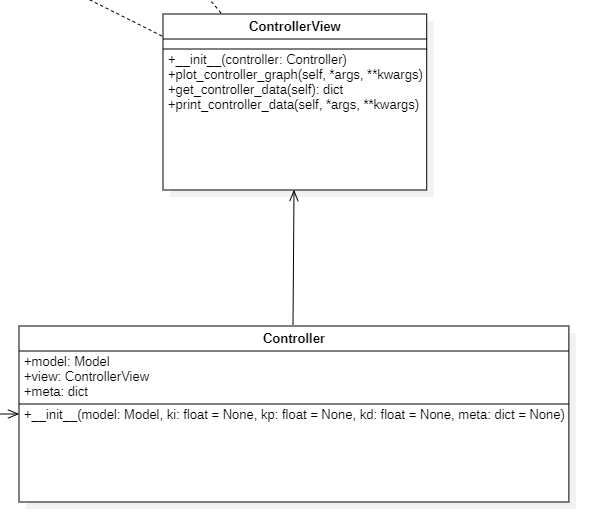
\includegraphics[scale=0.7]{figuras/class_diag_controller}
    \label{fig:class_diag_controller}
    \\
    \vspace{0cm}\hspace{0cm}\small{Fonte: Do autor}
\end{figure}

\begin{figure}[H]
    \centering
    \caption{Diagrama de classes ampliado - BaseControllerAproximation}
    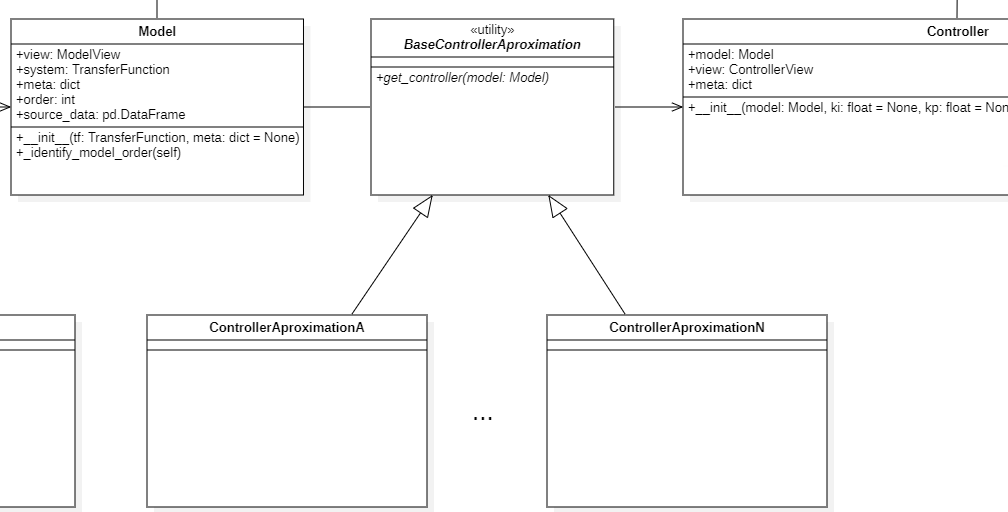
\includegraphics[scale=0.6]{figuras/class_diag_bcacontroller}
    \label{fig:class_diag_bcacontroller}
    \\
    \vspace{0cm}\hspace{0cm}\small{Fonte: Do autor}
\end{figure}

\section{Descrição do ambiente de implementação}

Nesta sessão serão explorados itens referentes ao ambiente de implementação utilizado para o
desenvolvimento, todos visando necessidades para implementação e publicação da biblioteca ou boas práticas de
desenvolvimento.

Para possibilitar a manutenção do código e facilitar futuras implementações é necessária a adoção de uma
estrutura de código e pastas que seja comum a comunidade, além disso existe a necessidade de uma estrutura compatível
com a publicação do código da biblioteca e do isolamento do código fonte da biblioteca dos testes da mesma.
Com isso em mente, foi adotada a estrutura apresentada em \cite{auto_test_vid}, que atende a essas necessidades.

\subsection{Controle de versão}

Foi escolhido o Git como opção de sistema de controle de versões da biblioteca.
Ele é um sistema de controle de versões preferido da comunidade, devido a sua alta performance, natureza decentralizada
e funcionalidades robustas para manipulação de grandes projetos \cite{usegit}.
Além de ser gratuito e de código aberto, é amplamente utilizado e integrado em um pletora de ferramentas e repositórios
como GitHub.

\subsection{Verificações e Testes}

Nesta sessão será abordado o uso de ferramentas de verificação de código como Mypy e Flake8, bem como ferramentas
que foram utilizadas para automação de testes, como Pytest, tox e GitHub actions.

\subsubsection{Mypy e Flake8}
Ambas as ferramentas Mypy e Flake8 foram utilizadas durante o desenvolvimento para verificar erros de tipagem e
adequação ao PEP 8, de forma que o resultado final passa nas verificações de ambas as ferramentas.
Elas também foram adicionadas ao processo de automação de testes descrito em \ref{subsubsec:devtox}, para que não
ficassem apenas a cardo do uso manual pelo desenvolvedor.

\subsubsection{Pytest}

Para cada uma das classes implementadas foram desenvolvidos testes unitários, para validação de suas funcionalidades e
garantia de que implementações futuras que alterem os resultados de funcionalidades já implementadas, possivelmente de
forma incorreta, não passem despercebidas gerando falhas ao rodar os testes.

\subsubsection{tox}\label{subsubsec:devtox}

A ferramenta tox foi utilizada para automatizar a execução das verificações, com Mypy e Flake8, e testes unitários, com
PyTest, para as versões 3.9 e 3.10 do Python.
De forma que ao roda-lo, com base no arquivo de configuração criado, são instaladas as dependências do projeto em um
ambiente virtual e são executadas todas as verificações e testes.

\subsubsection{GitHub Actions}

Foi utilizada a plataforma de CI/CD do GitHub, GitHub Actions para a criação de um workflow de testes, que roda a
ferramenta tox descrita em \ref{subsubsec:devtox}, em ambientes Windows e Linux, toda vez que um pull é feito em uma
branch ou que é realizado um merge request.
Desta forma é automatizado o processo de testagem em diversos ambientes, que pode ser mais demorado e atrapalhar o
fluxo de desenvolvimento.
Além de garantir que os testes sejam sempre rodados para toda alteração que for feita no repositório.

\subsection{Documentação do código}

A documentação de código foi desenvolvida juntamente as implementações de cada classe.
Optou-se pelo uso da ferramenta Sphinx para a documentação de código utilizando o tema do projeto Read the Docs, onde
também foi hospedada como um projeto de código aberto e seguindo uma estrutura de documentação similar a da
biblioteca Python Control Systems Library.

\subsubsection{Sphinx}

Para a documentação em Sphinx foram desenvolvidas diversas páginas em reStructuredText tratando dos seguintes itens:
\begin{alineas}
    \item \textbf{index}: Página principal da documentação com breve introdução e sumário da documentação;
    \item \textbf{Sobre}: Visão geral do projeto e guia de instalação;
    \item \textbf{Introdução}: Início rápido com exemplos e explicações práticas, e explicação geral do funcionamento da biblioteca;
    \item \textbf{Referência de Classes}: Listagem de todas as classes implementadas com breve resumo para cada grupo de classes;
    \item \textbf{Referências}: Página de glossário e referências bibliográficas utilizadas na documentação;
    \item \textbf{Desenvolvimento}: Página com orientações ao desenvolvimento.
\end{alineas}

Além disso a documentação de todas as classes e métodos implementados foi feita juntamente ao código fonte, através de
docstrings suportadas que foram interpretadas pelo Sphinx, que gerou páginas da documentação para cada classe, e essas
ficaram facilmente acessíveis através da página de referência de classes.

Algumas extensões foram adicionadas ao projeto para facilitar a documentação e melhorar a visualização e usabilidade:

\begin{alineas}
    \item \textbf{autodoc}: Utilizada para gerar documentação automaticamente baseado nas docstrings;
    \item \textbf{intersphinx}: Possibilita links entre documentações de diferentes bibliotecas;
    \item \textbf{mathjax}: Suporte a expressões matemáticas no formato LaTex;
    \item \textbf{autosummary}: Utilizada para gerar sumários de documentação automaticamente baseado nas docstrings;
    \item \textbf{napoleon}: Facilidade de sintaxe nas docstrings;
    \item \textbf{numpydoc}: Facilidade de sintaxe nas docstrings;
    \item \textbf{linkcode}: Adiciona link direto da documentação para o código fonte no repositório;
    \item \textbf{sphinx\_paramlinks}: Possibilita referencias parâmetros nas docstrings;
    \item \textbf{bibtex}: Suporte a referências do tipo BibTex;
    \item \textbf{sphinx\_rtd\_dark\_mode}: Modo escuro para o tema Read the Docs.
\end{alineas}

\subsubsection{Read the Docs}

Foi optado pelo uso do tema do projeto Read the Docs por questões gostos visuais e facilidade de navegação pela
documentação.
Além disso, foi utilizada a hospedagem gratuita para projetos de código aberto e da comunidade fornecida pela Read the
Docs.
Uma integração com o repositório git é fornecida para que toda vez que a branch principal for atualizada no repositório
a documentação no Read the Docs também seja atualizada automaticamente.

A documentação de código pode ser acessada por qualquer um na íntegra pelo link disponível no apêndice \ref{ch:actdocs}.

\subsection{Disponibilização do código}

Nesta sessão são descritas as formas como o código foi disponibilizado para uso, leitura e sugestões de melhoria.

\subsubsection{GitHub}

Visando disponibilizar o código fonte como código aberto e acessível, foi criado um repositório público e gratuito na
plataforma GitHub, cujo link pode ser encontrado no apêndice \ref{ch:actgithub}, onde qualquer um pode ter acesso a todo
o código fonte desenvolvido, bem como apontar bugs e sugerir alterações.

\subsubsection{PyPI}

Após a conclusão do desenvolvimento da biblioteca, iniciou-se o processo de disponibilização no PyPI\@.
Para isso foram criados arquivos de configuração do projeto, com detalhes como nome, versão, autor e requerimentos
para instalação.
Por fim o pacote foi carregado o PyPI utilizando a ferramenta twine, garantindo um upload seguro.
Este processo tornou o a biblioteca acessível para instalação via pip para qualquer pessoa.

\section{Implementação}
Esta seção detalha a implementação do código-fonte principal, contendo todas as funcionalidades disponibilizadas a
usuários dela.
Da mesma forma que na documentação da biblioteca as subseções desta seção representam grupos de classes implementadas
com paralelos diretos aos diagramas apresentados na seção \ref{sec:descarc}.

\subsection{Modelo}

Classes de modelo, representativas do Modelo matemático de uma planta de sistemas de controle.

\subsubsection{Model}

Classe representativa do Modelo matemático de uma planta de sistemas de controle.
Tipicamente o modelo matemático de uma planta no domínio da frequenica pode ser definido por um numerador e um
denominador em potências de $s$, como, por exemplo:
\begin{equation}
    \label{eq:modelex}
    P(s) = \frac{ s + 1 }{ s^2 + s + 1 }
\end{equation}

Essa classe funciona guardando um objeto de Função de Transferência (tf) da biblioteca de sistemas de controle do Python
(control), representando o modelo matemático de uma planta no domínio da frequenica, além de guardar alguns outros
metadados sobre a função de transferência, que poderão ser utilizados para identificação de modelo posteriormente,
por exemplo.

Além disso o atributo view, um objeto da classe ModelView possibilita a visualização de dados, estatísticas e gráficos
referentes a função de transferência.

Para ser instanciada, recebe um parâmetro tf, referente a função de transferência, e um parâmetro opcional source\_data
referente aos dados utilizados como base para gerar o modelo, caso o modelo tenha sido gerado dessa forma.

\subsubsection{ModelView}

Classe utilizada pra visualização de dados de um objeto da classe Model.

Esta classe recebe Model como parâmetro e tem como foco a visualização dos dados do mesmo.
Para as apresentações visuais, faz uso dos métodos explorados em \ref{subsec:dataviz}, e implementa os seguintes
métodos para possibilitar essa visualização são implementados:
\begin{alineas}
    \item \textbf{plot\_model\_step\_response\_graph}: Realiza a plotagem do gráfico da resposta a sinal degrau do
    Modelo, bem como as retas de tempo de acomodação, sobressinal, e valor de regime e os dados discretos caso tenham
    sido informados;
    \item \textbf{get\_model\_step\_response\_data}: Utiliza control.step\_info da biblioteca de controle para
    obtenção dos dados de resposta a sinal degrau do Sistema no formato de dicionário do Python;
    \item \textbf{print\_model\_step\_response\_data}: Imprime em tela os dados de resposta a sinal degrau do sistema;
    \item \textbf{print\_tf}: Imprime em tela a função de transferência do modelo, com formatação matemática caso
    esteja sendo executado em ambiente Jupyter.
\end{alineas}

\subsubsection{FirstOrderModel}

Essa classe é voltada um Modelo paramétrico da dinâmica de um processo comumente encontrado na indústria,
caracterizado pela função de transferência \eqref{eq:firstordertf} detalhado em \ref{subsec:modelfund}. Sendo uma
subclasse de Model, essa classe adiciona suporte a definição de um modelo com os parâmetros K ($K$), tau
($\tau$) e theta ($\theta$) mas ainda mantém todas as funcionalidades da classe pai. Adicionalmente, ela faz uso do
atributo pade, caso $\theta$ seja diferente de zero.
Nele é salva a aproximação de padê para o atraso do sistema.

\subsection{Métodos de Identificação}

Classes de Identificação são subclasses de BaseModelIdentification, e implementam o método get\_model, que faz a
identificação de dados discretos de resposta a sinal degrau de um sistema de controle e retorna objeto da classe Model
ou de uma de suas subclasses.

\subsubsection{BaseModelIdentification}
Classe abstrata que serve de base para identificação de modelos (Model).
Classes de métodos de identificação de modelos devem ser subclasses desta classe.
Elas também devem implementar o método get\_model para retornar um objeto da classe Model que represente o modelo
matemático do sistema que produziu os dados recebidos.

Em geral, implementações farão a Identificação com base nos dados de resposta a sinal degrau.
Para tanto, o método get\_data\_input\_layout oferece um leiaute para serem informados os dados referentes a resposta
do Sistema a um sinal degrau em relação ao tempo.
Implementações de get\_model podem ler os dados e aplicar seus métodos de identificação específicos.

\subsubsection{ZieglerNicholsModelIdentification}

Esta é uma subclasse de BaseModelIdentification que implementa o método de identificação de Ziegler e Nichols, descrito
em \ref{subsubsec:znfun}.
Ela sobreescreve o método abstrato da classe pai get\_model, implementando para que, com base nos dados de resposta a
sinal degrau fornecidos e em outros parâmetros opcionais, sejam calculados os parâmetros para instanciar um objeto da
classe FirstOrderModel:

\begin{alineas}
    \item Utiliza DataInputUtils.get\_model\_data\_default para obter a tabela (pandas.DataFrame) com os dados de
    resposta do modelo;
    \item Então obtém a pandas.Series tf\_data (lista cujo index representa o tempo e os valores a saida)
    e o valor do sinal degrau através do método DataUtils.setup\_data\_default;
    \item Obtém o valor de regime e o momento de entrada em valor de regime através do método
    DataUtils.get\_vreg;
    \item Obtém o valor da inclinação da reta tangente e o momento em que a reta encosta na curva $y(t)$
    através do método DataUtils.get\_max\_tan;
    \item Encontra o valor de $y(t)$ quando $t$ é igual ao momento em que a reta encosta na curva $y(t)$;
    \item Utiliza a inclinação da reta tangente e a localização do ponto de encontro dela com a curva $y(t)$
    para encontrar os valores de $t_1$ e $t_3$ através do método
    DataUtils.get\_time\_from\_inclination e dos valores de $y(t)$ referentes aos pontos desejados,
    $y(t) = 0$ e $y(t) = y_f$, respectivamente;
    \item Obtém $K$ dividindo o valor de regime, $y_f$, pelo valor do sinal degrau;
    \item Com os valores de $t_1$ e $t_3$ em mãos calcula o valor de tau e theta,
    sendo $\tau = t_3 - t_1$ e $\theta = t_1$`;
    \item Dependendo do valor de theta e do parâmetro ignore\_delay\_threshold zera o valor de theta;
    \item Instancia um objeto da classe FirstOrderModel com os valores obtidos.
\end{alineas}

\subsubsection{HagglundModelIdentification}

dev identificação Hagglund

\subsubsection{SmithModelIdentification}

dev identificação Smith

\subsubsection{SundaresanKrishnaswamyModelIdentification}

dev identificação Sundaresan Krishnaswamy

\subsubsection{NishikawaModelIdentification}

dev identificação Nishikawa

\subsection{Controlador}

dev Implementaçãp do Controlador

\subsubsection{Controller}
\subsubsection{ControllerView}

\subsection{Métodos De Aproximação de Controlador}

dev Metodos De Aproximação De Controlador

\subsubsection{BaseControllerAproximation}

\subsubsection{Aproximação de ganhos de controlador para modelos de primeira ordem por tabela}
FirstOrderTableControllerAproximation
FirstOrderTableControllerAproximationItem

\subsubsubsection{ZieglerNicholsControllerAproximation}

dev aproximação de ganhos Ziegler Nichols

\subsubsubsection{CohenCoonControllerAproximation}

dev aproximação de ganhos Cohen Coon

\subsection{Visualização de Dados}\label{subsec:dataviz}

dev Visualização dos Dados

\subsection{Manipulação de Dados}

dev datamanip